% !TEX root = ./report.tex

\clearpage
\section{The Inliner}
\label{sec:scheme}

Our inliner, written in C++, utilizes Jive integrations, and is compiled with
Jive. This section details the actions performed by the inliner, and the
reasoning behind these. First we list the action the inliner performs, before we
go more into depth on the reasoning behind them.

The following heuristic is executed by the inliner of this project when given an
RVSDG as input:

\begin{enumerate}
	\item For all recursive environments ($\phi$-regions):

	\begin{enumerate}
		\item Use the approach described in
Section~\ref{sub:scheme:inlining_recur_apply_nodes} to fill a list \textit{loop
breakers}. These functions ($\lambda$-nodes) are \textit{not} to be inlined.
		\label{MakeLoopBreakerListItem}
	\end{enumerate}

	\item Scan through the RVSDG, finding all call sites (\applyNode s). Exclude
all function calls to loop breakers, calls invoking functions which are not
statically known, or external functions.
	\label{ScanForApplyNodesItem}

	\item Make a list of the \applyNode s found in
Step~\ref{ScanForApplyNodesItem}, and order the list according to the heuristics
discussed in Section~\ref{sub:scheme:ordering_apply_nodes}. The order of
\applyNode s inlined can affect the total amount of \applyNode s inlined, even
when all of the \applyNode s are evaluated with the same heuristic.
\label{OrderApplyNodesFoundItem}

	\item Look at each \applyNode~in turn from the list made in
Step~\ref{OrderApplyNodesFoundItem} and decide whether or not to inline it
according to the heuristic discussed in
Section~\ref{sub:scheme:inlining_apply_nodes}:
	\label{LookAtNextCallSiteItem}

	\begin{enumerate}
		\item If the \applyNode~is inlined, add any newly copied (inlined)
\applyNode s, following the same criteria as used in
Step~\ref{ScanForApplyNodesItem}, to the list of \applyNode s. Continue with
Step~\ref{OrderApplyNodesFoundItem}.

		\item If the \applyNode~is not inlined, continue with
Step~\ref{LookAtNextCallSiteItem}, evaluating the next \applyNode .
		\label{InlineCallSiteItem}
	\end{enumerate}

	\item When the inliner reaches the end of the list, no more \applyNode s
have been inlined, and the inliner is finished.
\end{enumerate}

\subsection{Deciding which recursive functions to inline}
\label{sub:scheme:inlining_recur_apply_nodes}

The inliner visits all \applyNode s invoking statically known functions in the
RVSDG given as input, whether they invoke a recursive function or not. Before
the inliner collects any \applyNode s, it first finds all the $\phi$-regions in
the RVSDG. In each $\phi$-region, the call graph made by the $\lambda$-node's
\applyNode s inside always make a Strongly Connected Component (SCC).

Hence, for each $\phi$-region, the inliner chooses one $\lambda$-node, and
performs the following steps:

\begin{enumerate}
	\item Mark the $\lambda$-node as ``visited''.

	\item Collect all the \applyNode s contained within this $\lambda$-node.

	\item If one of the collected \applyNode~invokes another $\lambda$-node from
within the same $\phi$-region, check if the $\lambda$-node is marked as
``visited'':
	\begin{enumerate}
		\item If the invoked $\lambda$-node is marked as ``visited'', add it to
the list of \textit{loop breakers}.

		\item If the invoked $\lambda$-node is \textit{not} marked as
``visited'', recursively perform the steps of this list on that $\lambda$-node.
	\end{enumerate}
\end{enumerate}

In this manner it is guaranteed, by virtue of the SCC the call graph inside a
$\phi$-region makes, that all $\lambda$-nodes are visited. It is also guaranteed
that for every cycle in the SCC, there is at minimum \textit{one} $\lambda$-node
marked as a loop breaker. As such, the inliner knows which recursive functions
it must never attempt to inline, so as to ensure termination of the compilation.
The remaining $\lambda$-nodes residing in $\phi$-regions not marked as loop
breakers may then be inlined according to the same criteria as any non-recursive
function.


\unsure{Put a reference to Section~\ref{sub:fw:optimal_loop_breakers} here?}
While there are better ways~\cite{BasMscThesis} to choose loop
breakers\footnote{So as to minimize the amount of loop breakers per cycle in the
$\phi$-region.}, we unfortunately did not have the time to implement one for
this project.

\subsection{The order of call sites inlined}
\label{sub:scheme:ordering_apply_nodes}

The order in which the \applyNode s inlined are inlined, can make a difference
for not only \textit{how many} \applyNode s are inlined, but also \textit{which}
that get inlined. To illustrate this, let us give the reader the following
example.

As mentioned, the heuristic deciding whether or not to inline a specific
\applyNode~is the same for all the \applyNode s collected from the RVSDG given
as input to the inliner. Hence, if the heuristic deciding whether an
\applyNode~is inlined or not depends upon whether the \textit{internal node
count} of the function it invokes is less than four, the example illustrated by
Figure~\ref{fig:inline_ordering_ex} will either inline \textit{both} of the
depicted \applyNode s, or just one of them.

\begin{figure}[H]
	\centering
	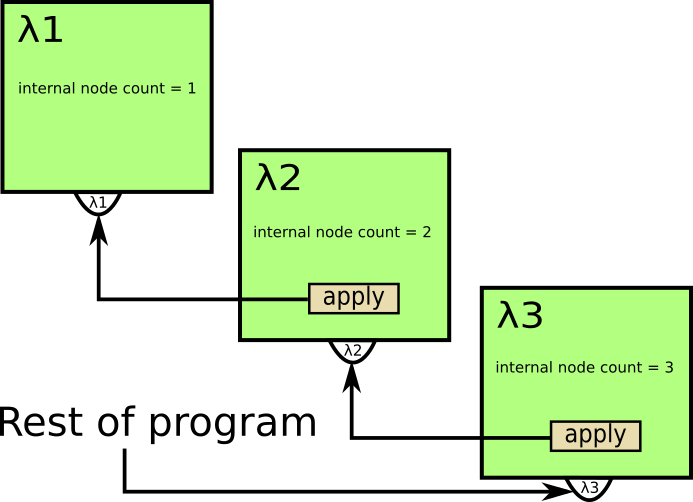
\includegraphics[width=0.75\textwidth]{figures/inline_ordering_ex}
	\caption{A minimal example of an RVSDG subgraph, depicting a function call
order in a program.}
	\label{fig:inline_ordering_ex}
\end{figure}

If the inliner evaluates the \applyNode s in Figure~\ref{fig:inline_ordering_ex}
in a top-down order, $\lambda_1$ can be inlined into $\lambda_2$. The newly
created $\lambda_{1-2}$ with an internal node count of $3$ can be inlined into
$\lambda_3$, resulting in all of them being inlined into a new single function;
$\lambda_{1-2-3}$.

However, if the inliner evaluates the \applyNode s in
Figure~\ref{fig:inline_ordering_ex} in a bottom-up order instead, $\lambda_3$
can be inlined into $\lambda_2$. But the newly created function
$\lambda_{2-3}$'s amount of nodes contained within exceeds 3, and can hence not
be inlined into $\lambda_1$.

\textit{This constructed example assumes the node count contained within each
function created by inlining to be the sum of the itnernal node counts of the
original function and the one inlined. In other words, no optimizations or other
compiler techniques are assumed performed on the RVSDG during the traversal of
the \applyNode s, or before/after each inlining.}

As our constructed example shows, the order in which the \applyNode s being
inlined are visited matter. Because of this, our inliner is able to traverse the
\applyNode s of the RVSDG given as input in either a top-down order, or a
bottom-up order. Section~\ref{sub:fw:call_site_visit_order} discusses
ideas for potential work for future research regarding the impact of the order
of inlined call sites.

\subsection{Inlining a call site}
\label{sub:scheme:inlining_apply_nodes}

While there exist several~\cite{GHCPaper,AdaptvStratInlSubst} ways in
literature in which inlining is performed, we decided upon our chosen
approach~\cite{AdaptvCompilAndInlingWaterman} because it permits effective
testing for an apt heuristic when deciding on whether or not to inline a call
site.

As mentioned, all \applyNode s eligible for inlining get inlined based on the
same heuristic per run of our inliner. The heuristic is based on \textit{Inliner
Conditions} (ICs), such as the following:

%\begin{multicols}{3}
\begin{itemize}
	\item \textit{Node Count} (NC)

The amount of nodes (operations) contained within the function invoked by the
\applyNode .

	\item \textit{Loop Nesting Depth} (LND)

The amount of nested loops the \applyNode~resides within.

	\item \textit{Static Call Count} (SCC)

The total amount of \applyNode s invoking the same function in the RVSDG given
as input.
\end{itemize}
%\end{multicols}

These ICs and others described in Section~\ref{sub:meth:inlining_conditions}
allow us to write and re-write the inlining heuristic effectively, by letting us
write them using \textit{Conjunctive Normal Form} (CNF). Thus, the CNFs written
for our inliner heuristic are written in the following fashion:
\lstinline"(NC < X || SCC < Y || (SCC < Z && LND > W))", where \lstinline!X!,
\lstinline!Y!, \lstinline!Z!, and \lstinline!W! are placeholder variables.

While the work of Waterman~\cite{AdaptvCompilAndInlingWaterman}, which our
approach is based upon, utilizes a hillclimber algorithm to find the most
optimal values for the placeholder variables for each individual program, we did
not have sufficient time to implement a hillclimber algorithm in this project.

Still, while the placeholder variables used in our CNFs need to be hardcoded for
each run of our inliner, this approach still permits us to search the parameter
space for decent parameters for the inlining heuristic.
